\begin{wrapfigure}[42]{R}{10cm}
	%	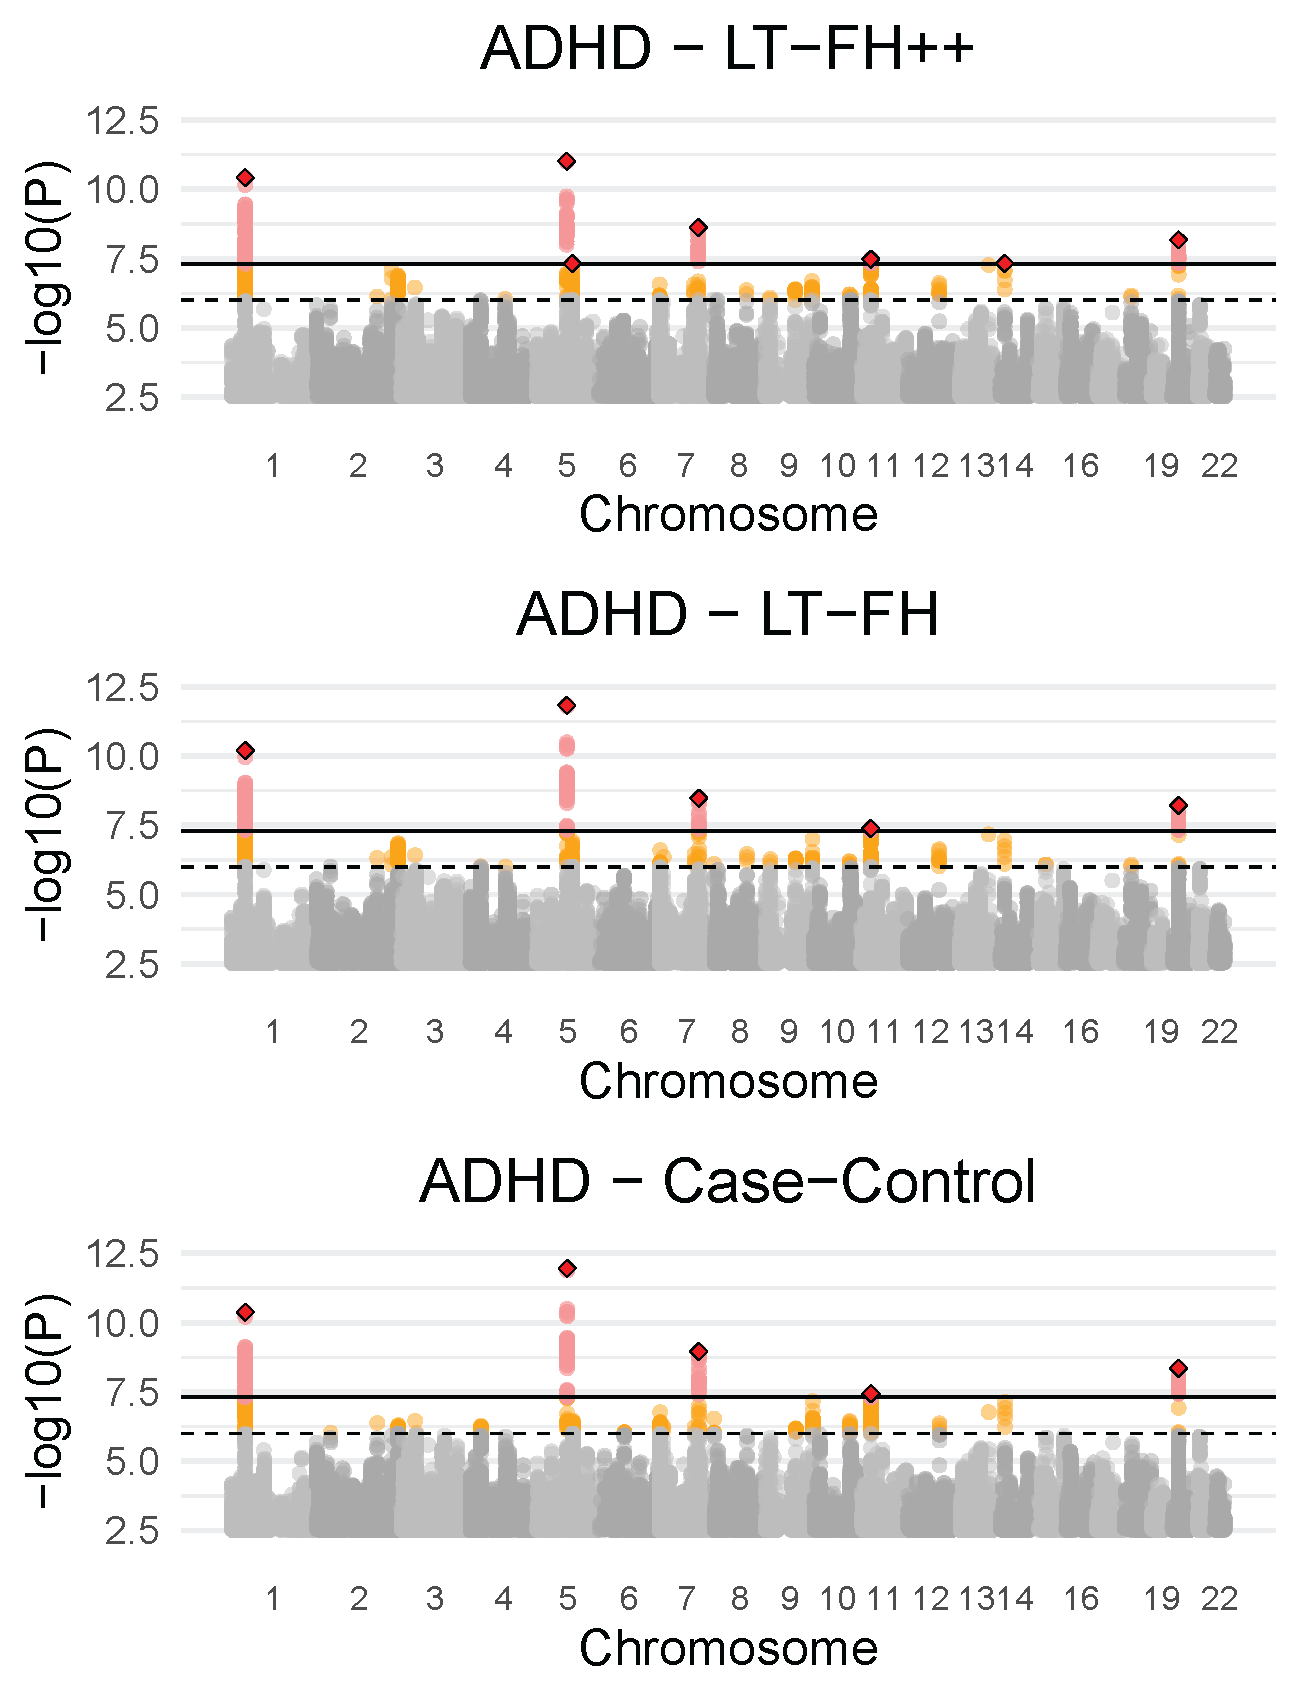
\includegraphics[width=0.7\textwidth]{results/manhattanPlot_ADHD.pdf} % adds a lot of loading 
	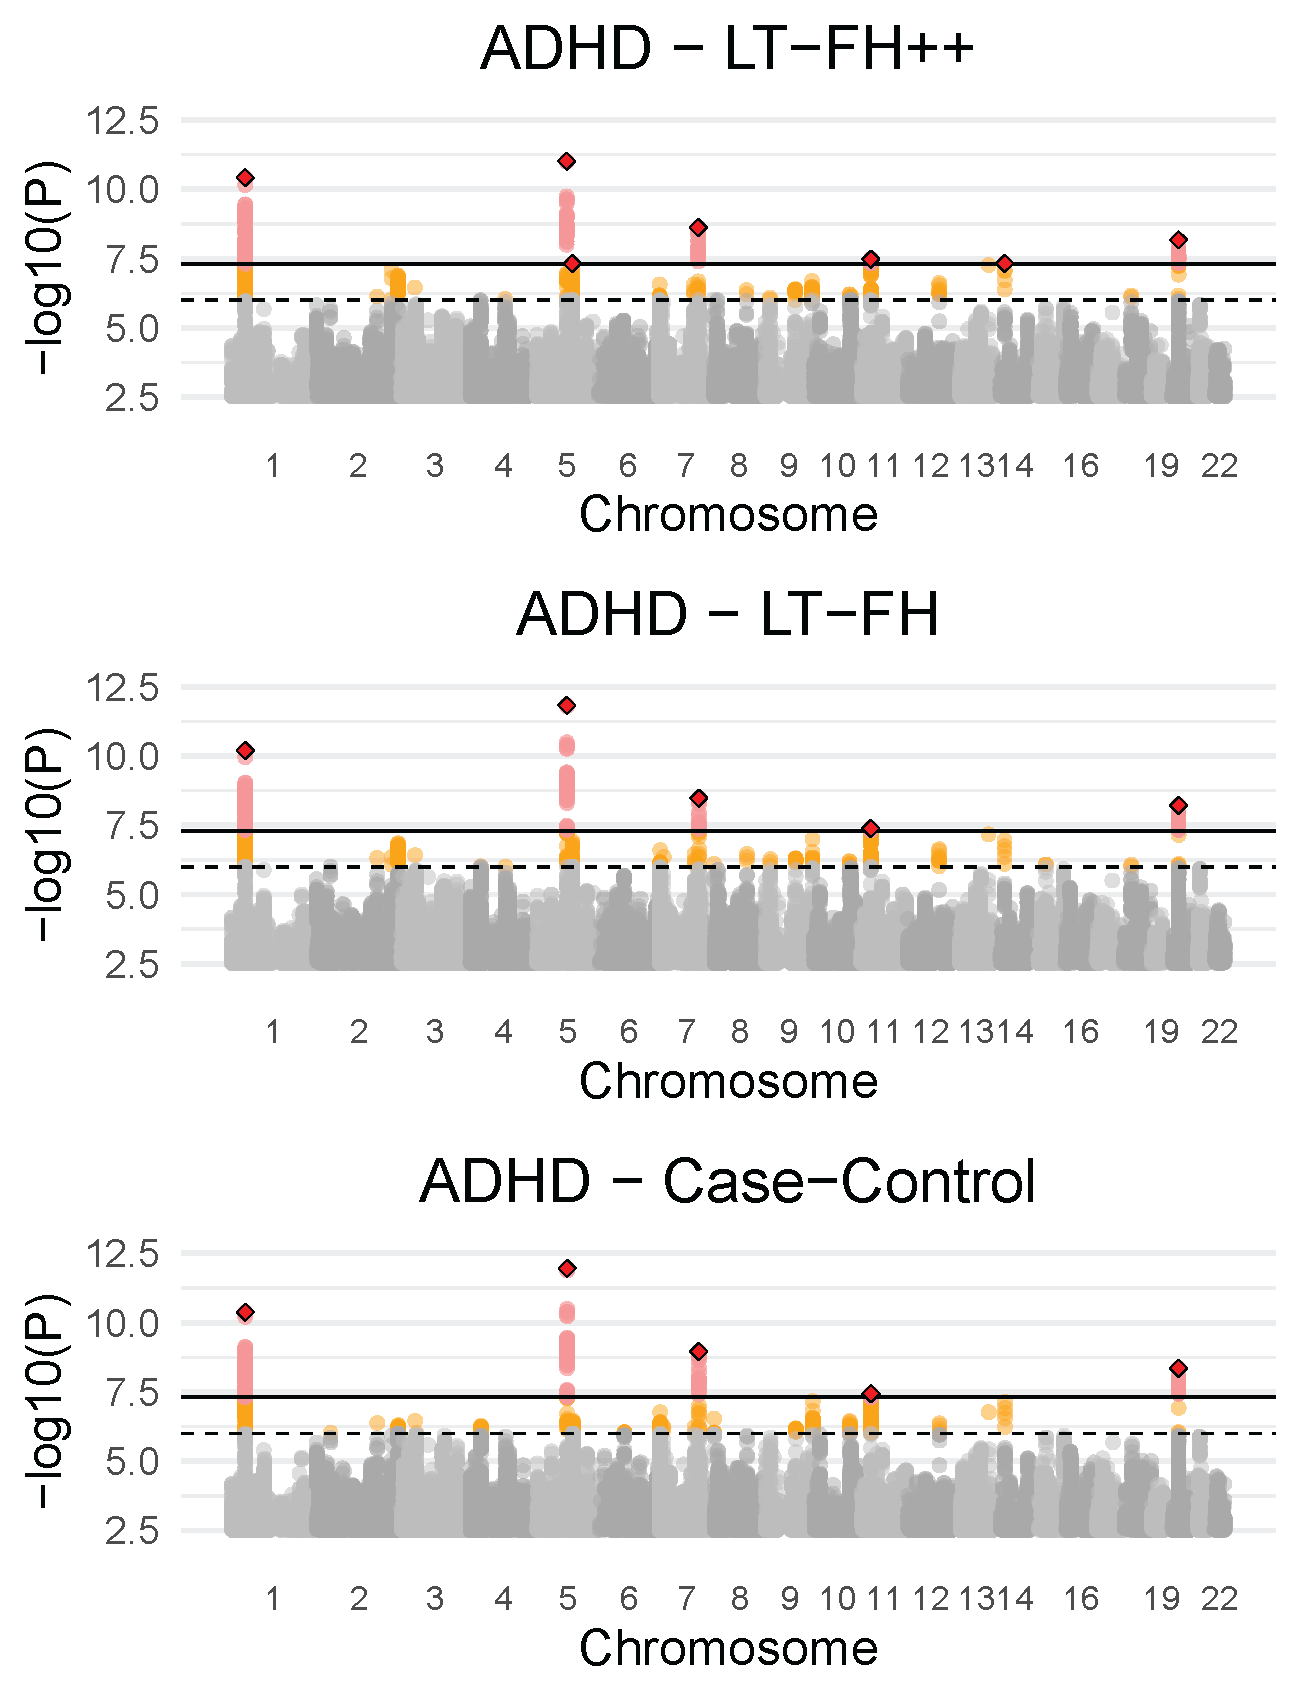
\includegraphics[width=10cm]{results/manhattanPlot_ADHD.png}
	\caption[Manhattan plots for LT-FH++, LT-FH, and case-control GWAS of ADHD in the iPSYCH data]{
		\sl The dashed line indicates a suggestive p-value of $ 5\times 10^{-6} $ and the fully drawn line at $ 5\times 10^{-8} $ indicates genome-wide significance threshold. The genome-wide significant SNPs are coloured in red. The diamonds correspond to top SNPs in a window of size $ 300,000 $ base pairs. Originally Figure $ 5 $ from Paper $ 1 $\cite{pedersen2022accounting} (also \cref{app:ltfhpp}, Figure $ 5 $)}	
	\label{fig:LTFH++_manhattanADHD}
\end{wrapfigure}

The second paper utilised the ADuLT model, which is the model underlying LT-FH++. The name change is in large part due to the focus on only the age-dependency and not family history, even though it is the same model. The purpose of the project was to examine the performance of the ADuLT outcome with established time-to-event GWAS methods that are based on the Cox proportional hazards (PH) model. It is two fundamentally different ways to approach time-to-event analysis in a GWAS setting. The adoption of Cox PH models in a GWAS setting has been limited, which has also been evident in the relative lack of method developments for Cox PH models compared to other regression models. Since one of the main limitations for Cox PH is the computational cost of such a model, GWAS with these models have been limited to less than $ 100,000 $ individuals. Recently, a method called SPACox \cite{bi2020fast} has been proposed that allows for far better scaling, and allowing for analysis of large biobanks. We will use SPACox as a representative of Cox PH models to compare to in this paper.
\newpage
\subsection{Simulation Results}

As for the first paper, we assessed the models in simulations first. We simulated the genotypes and assigned phenotypes with two generative models. The first model was the liability threshold model and the second model was the proportional hazards model. Notably, one would expect a method based on the liability threshold model to perform the best under this model, and subpar under other generative models. The simulation results shown in \cref{fig:adult_simulations} show the power for $ 10 $ replications under two different generative models and for different population prevalences. In \cref{fig:adult_simulations}A, the ADuLT or case-control status methods perform slightly better than the Cox PH model under the liability threshold model and vice versa, which is what we expected. Notably, there is no case ascertainment in those simulations. The results shown in \cref{fig:adult_simulations}B are with case ascertainment and we observe a large shift in power between methods under both generative models. In short, the simulation results show that the Cox PH based method has a far lower power than the LTM based methods under both generative models, when cases are ascertained. Even after performing inverse probability weighing Cox PH on a select subset of null SNPs and all causal SNPs, we observed the same result. This indicates that the Cox PH models with the current implementation suffers from a significant power loss when case ascertainment is present in a GWAS setting, which is very common in practice.

%\begin{wrapfigure}{O}{10cm}
\begin{figure}[h]
	\centering
	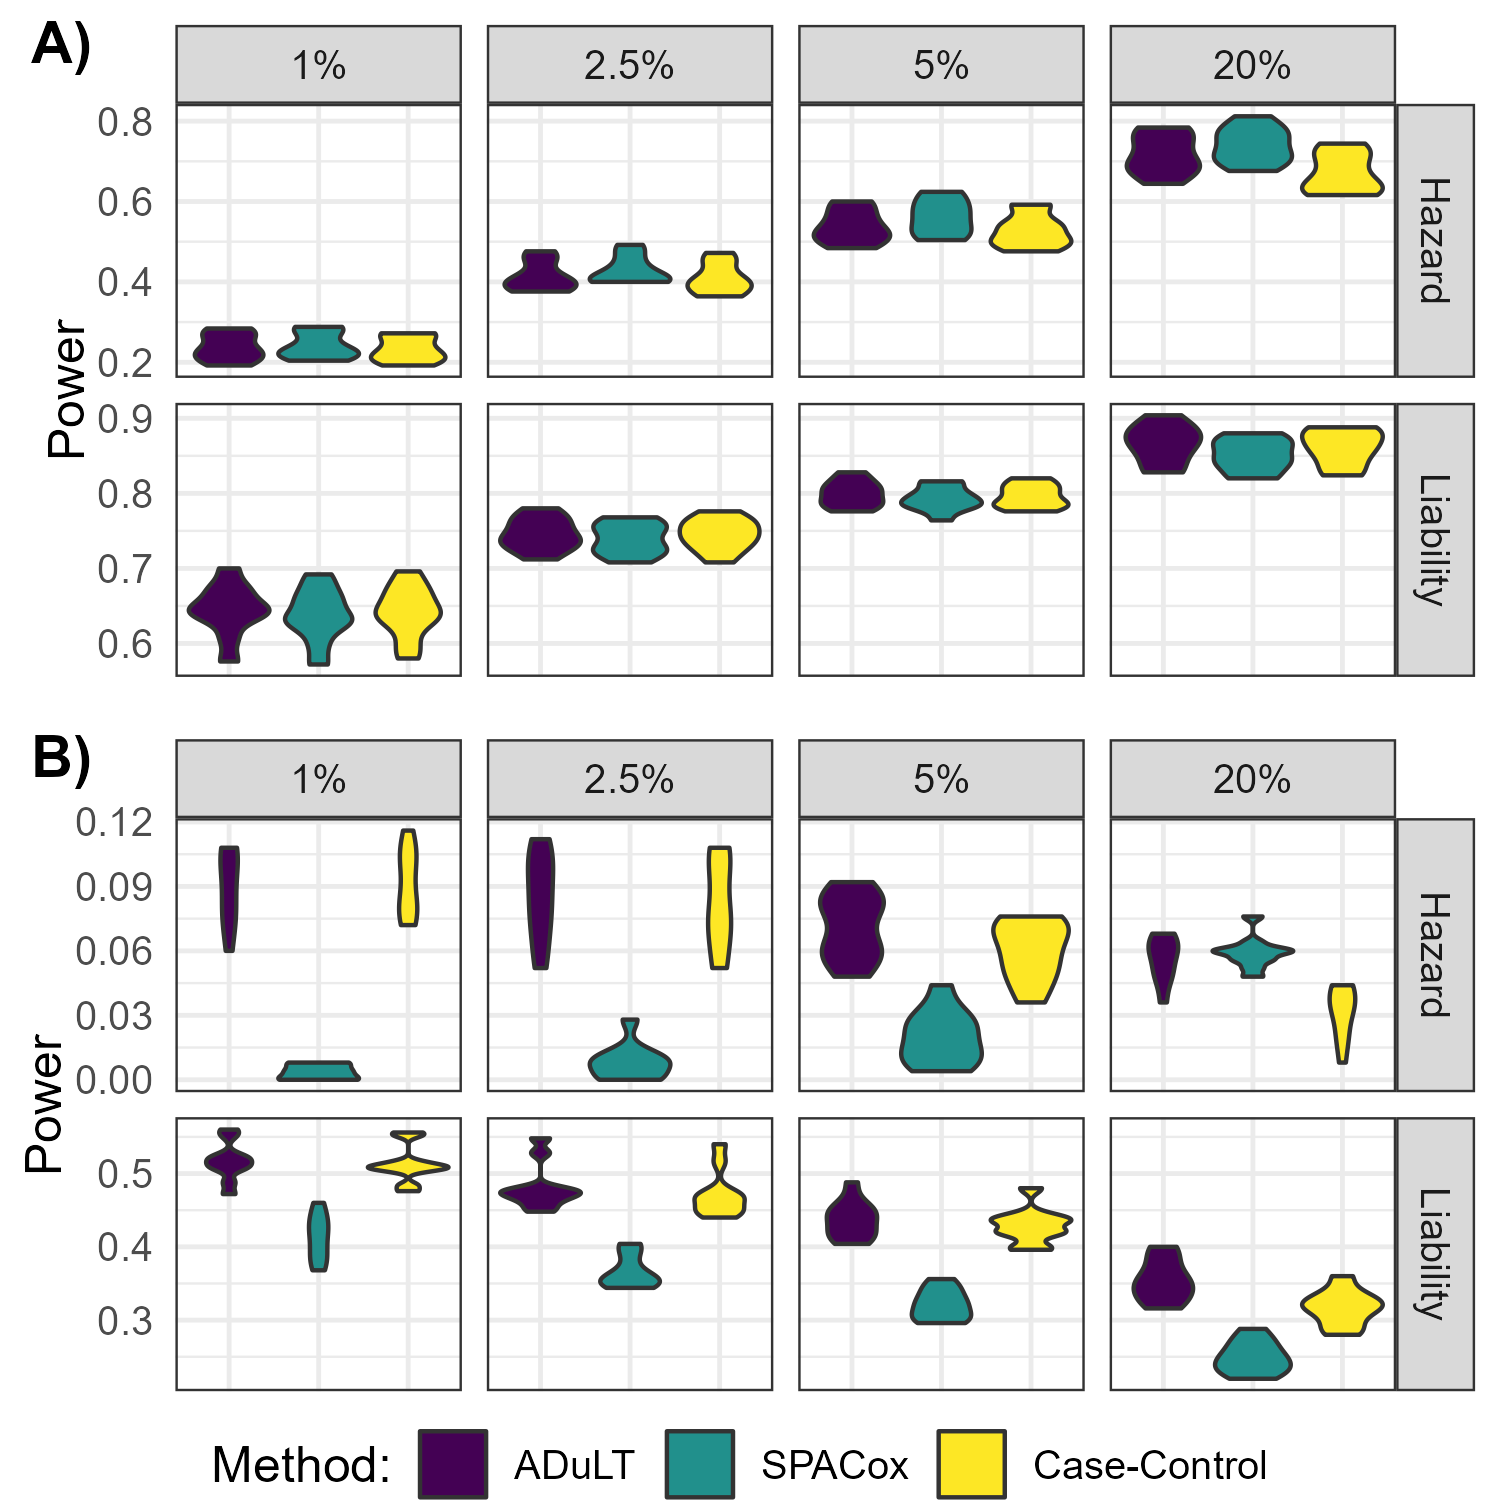
\includegraphics[width=10cm]{results/adult_combined_C250_power}
	\caption[Power simulation results with $ 250 $ causal SNPs under both generative models and varying prevalences.]{\sl Originally, Figure $ 2 $ in Paper $ 2 $\cite{pedersen2022adult} (also \cref{app:adult}, Figure $ 2 $) and provided as-is. The power is shown for different population prevalence, varying from $ 1\% $ to $ 20\% $. \textbf{A)} The power, i.e.\ the fraction of causal SNPs detected for each method, \textbf{without downsampling}. \textbf{B)} The power \textbf{with downsampling}, i.e.\ the number of individuals is subsampled to $ 10,000 $ cases and $ 10,000 $ controls.}
	\label{fig:adult_simulations}
	%\end{wrapfigure}
\end{figure}


\subsection{Real-World Analysis}
Next, we applied the same analysis to real-world data to assess whether we observed the same behaviour with case ascertainment present in the data. iPSYCH is particularly useful for this, as all cases in a given time period have been sampled and sequenced, meaning the iPSYCH data has a high case ascertainment.

We found that the Cox PH model had a rather large loss of power compared to ADuLT and case-control status. Across the four analysed psychiatric disorders, ADuLT found $ 20 $ independent associations, case-control status found $ 17 $, and SPACox found $ 8 $. The ADHD Manhattan plots for the three methods compared in paper 2 can be found in \cref{fig:adult_ADHD}. In no circumstances did the Cox PH model outperform a LTM based method, showing that the currently implementation of Cox PH model does not perform as well as simpler models such as linear regression, which are also far more computationally efficient.

%\begin{wrapfigure}{O}{10cm}
\begin{figure}[h] 
	\centering
	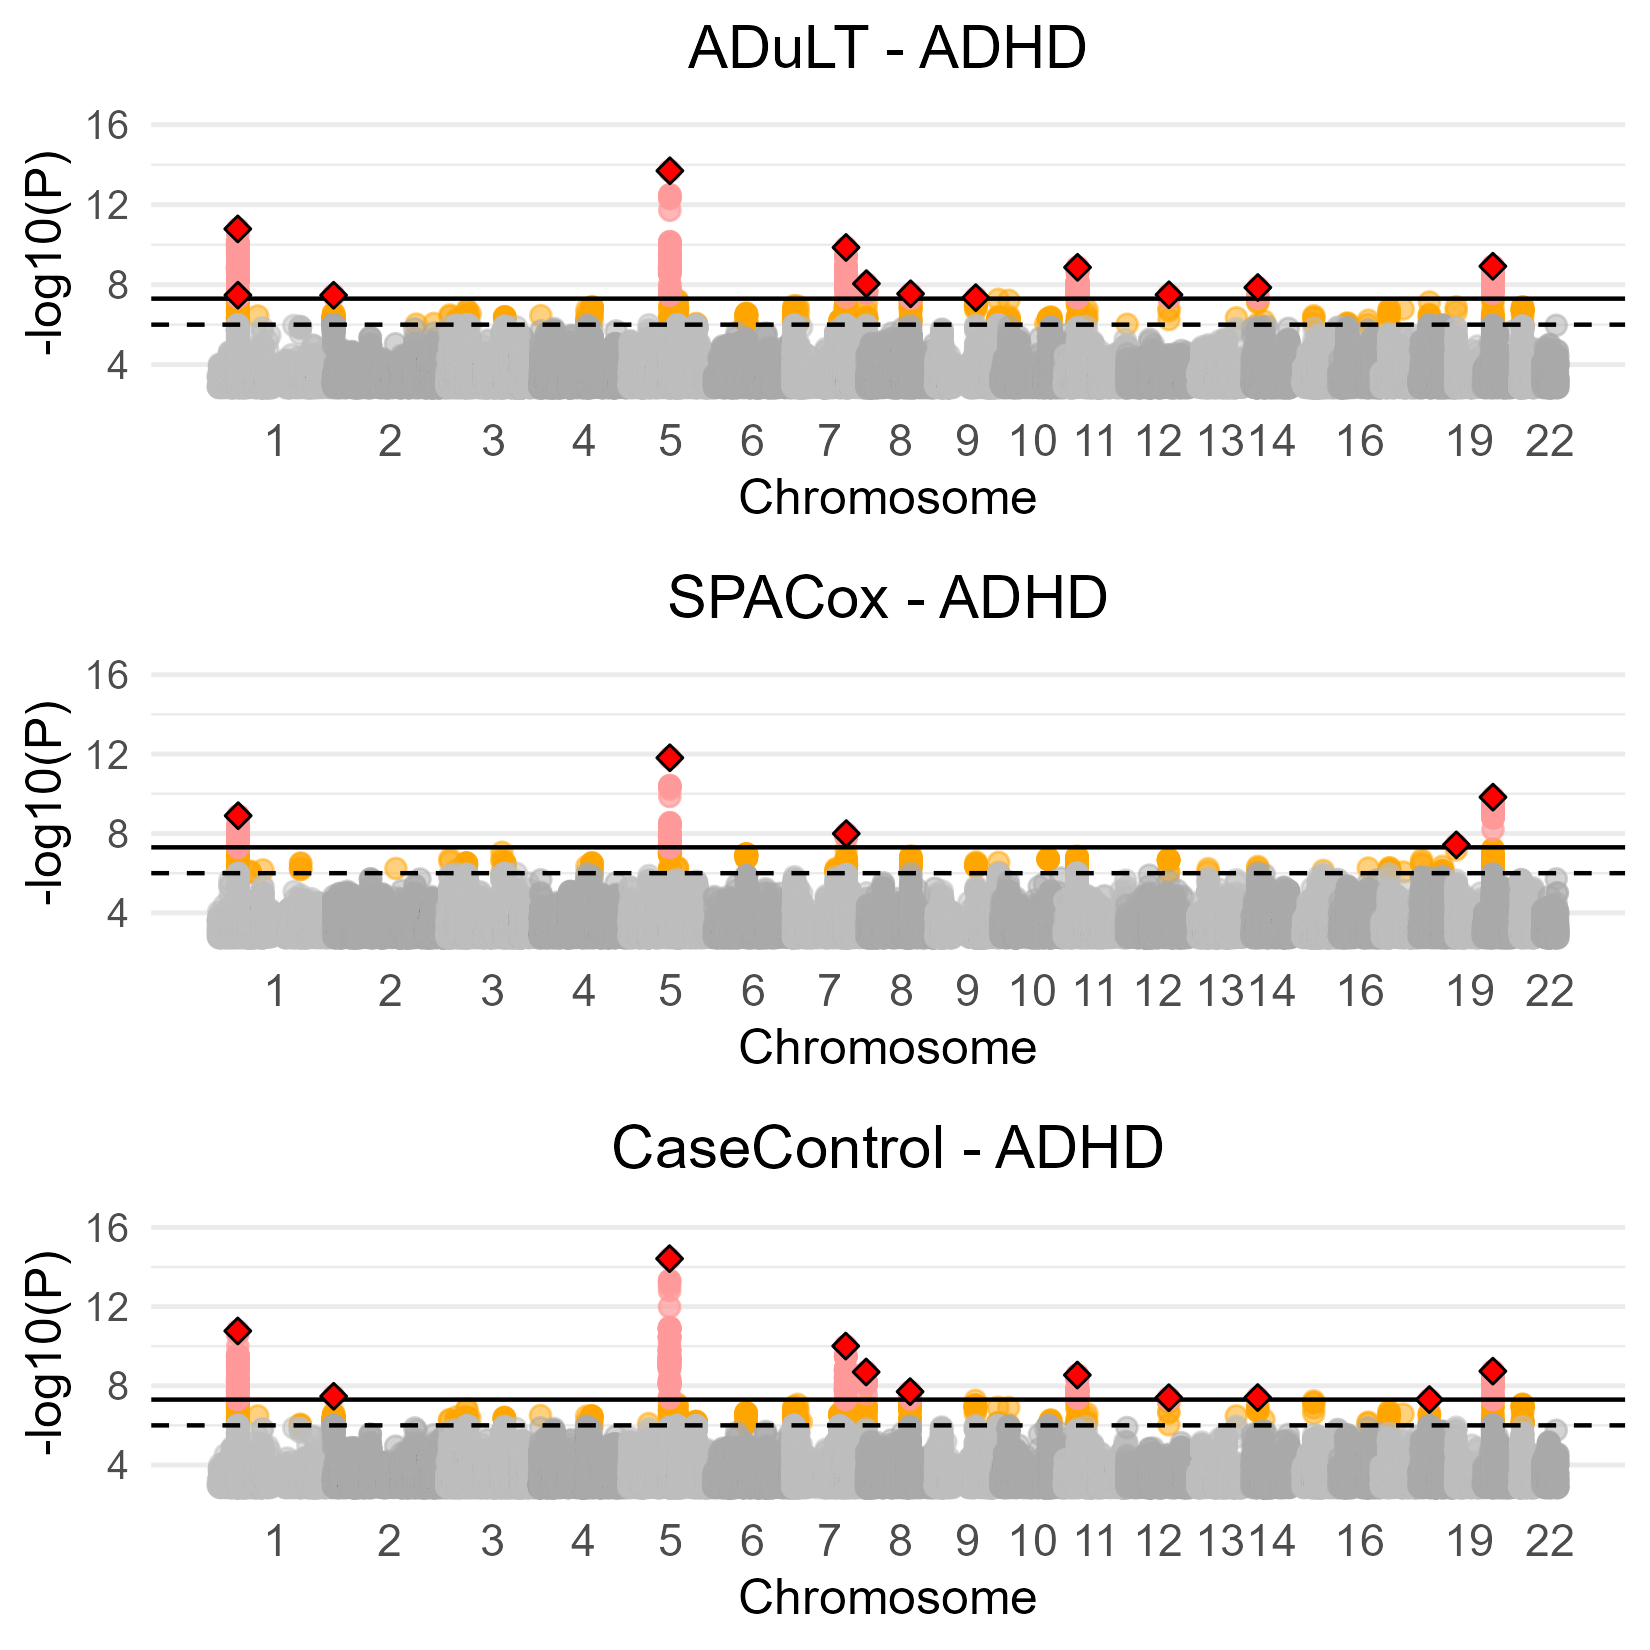
\includegraphics[width=10cm]{results/adult_manhattanPlot_ADHD}
	\caption[Manhattan plots from GWAS with the ADuLT phenotype, SPACox, and case-control status for ADHD]{
		\sl Manhattan plots for ADHD for all three methods. Case-control GWAS uses the age of individuals as a covariate, whereas the ADuLT GWAS and SPACox do not. The plot is originally from Figure $ 4 $ in Paper $ 2 $\cite{pedersen2022adult} (also \cref{app:adult}, Figure $ 4 $); it is provided as-is. The orange dots indicate suggestive SNPs with a p-value threshold of $ 5 \times 10^{-6} $. The red dots correspond to genome-wide significant SNPs with a p-value threshold of $ 5 \times 10^{-8} $. The diamonds correspond to the lowest p-value LD clumped SNP in a $ 500,000 $ base pair window with an $ r^2 = 0.1 $ threshold.}
	\label{fig:adult_ADHD}
%\end{wrapfigure}
\end{figure}

